%% -----------------------------------------------------------------
%% This file uses UTF-8 encoding
%%
%% For compilation use following command:
%% latexmk -pdf -pvc -bibtex --shell-escape thesis
%%
%% -----------------------------------------------------------------
%%                                     _     _      
%%      _ __  _ __ ___  __ _ _ __ ___ | |__ | | ___ 
%%     | '_ \| '__/ _ \/ _` | '_ ` _ \| '_ \| |/ _ \
%%     | |_) | | |  __/ (_| | | | | | | |_) | |  __/
%%     | .__/|_|  \___|\__,_|_| |_| |_|_.__/|_|\___|
%%     |_|                                          
%%
%% -----------------------------------------------------------------

\documentclass{kithesis}

% Additional packages
\usepackage[main=slovak,english]{babel}

\usepackage{listings}  % for source code
% Listings settings
% See for details: https://en.wikibooks.org/wiki/LaTeX/Source_Code_Listings
\lstset{
    basicstyle=\small\ttfamily,  % smaller typewriter font
    showstringspaces=false       % don't show spaces in string
}
\def\lstlistingname{Zdrojový kód}

% Variables
%\thesisspec{figures/thesisspec.png} 

\title{My thesis \br (the skeleton)}{Moja záverečná práca \br (šablóna)}

%\author{Janko Hraško}
\author[Bc.]{Janko}{Hraško}[PhD.]
\supervisor{Leslie Lamport} %veduci prace
\consultant{Donald E. Knuth} %konzultant
%\college{University of Žilina}{Žilinská univerzita} %univerzita
%\faculty{Faculty of Electrical Engineering and informatics}{Fakulta elektrotechniky a informatiky} %fakulta
%\department{Department of Computers and Informatics}{Katedra počítačov a informatiky} %katedra
%\departmentacr{DCI}{KPI} % skratka katedry
%\thesis{Master thesis}{Diplomová práca} %typ prace
\submissiondate{13}{5}{2018}
%\fieldofstudy{9.2.1 Informatika}
%\studyprogramme{Informatika}
%\city{Košice} %mesto
\keywords{\LaTeX, programming, typesetting}{\LaTeX, programovanie, sadzba textu}
%\declaration{som nepodvadzal}

\abstract{%
    % english 
	\blindtext
}{%
    % slovak 
	\blindtext
}

\acknowledgment{Na tomto mieste by som rád poďakoval svojmu vedúcemu práce za jeho čas a odborné vedenie počas riešenia mojej záverečnej práce.

Rovnako by som sa rád poďakoval svojim rodičom a priateľom za ich podporu a povzbudzovanie počas celého môjho štúdia.
    
V neposlednom rade by som sa rád poďakoval pánom \textit{Donaldovi E. Knuthovi} a \textit{Leslie Lamportovi} za typografický systém \LaTeX, s ktorým som strávil množstvo nezabudnuteľných večerov.}

% if you want to work only on selected chapters
%\includeonly{chapters/analyza} %,chapters/synteza}

% Load acronyms
% Acronyms
% ========
%
% An acronym is a word formed from the initial letters in a phrase. 
%
% Acronym Definition Exapmle:
% ---------------------------
% \newacronym{gcd}{GCD}{Greatest Common Divisor}
% \newacronym{dry}{DRY}{Don't Repeat Yourself}
%
% Usage:
% ------
% You can use these three options:
% 
% \acrlong{}  
%   Displays the phrase which the acronyms stands for. Put the label of the acronym inside the braces. In the example, \acrlong{gcd} prints Greatest Common Divisor. 
%
% \acrshort{} 
%   Prints the acronym whose label is passed as parameter. For instance, \acrshort{gcd} renders as GCD. 
%
% \acrfull{} 
%   Prints both, the acronym and its definition. In the example the output of \acrfull{dry} is Don't Repeat Yourself (DRY). 
% 
% For more information see:
% -------------------------
% * https://www.sharelatex.com/learn/Glossaries 
% * https://en.wikibooks.org/wiki/LaTeX/Glossary
%



%% -----------------------------------------------------------------
%%          _                                       _   
%%       __| | ___   ___ _   _ _ __ ___   ___ _ __ | |_ 
%%      / _` |/ _ \ / __| | | | '_ ` _ \ / _ \ '_ \| __|
%%     | (_| | (_) | (__| |_| | | | | | |  __/ | | | |_ 
%%      \__,_|\___/ \___|\__,_|_| |_| |_|\___|_| |_|\__|
%%                                                      
%% -----------------------------------------------------------------

\begin{document}
%% Title page, abstract, declaration etc.:
\frontmatter{}

%% List of code listings, if you are using package minted
%\listoflistings

%\pagenumbering{arabic}

%% Chapters
% !TEX root = ../thesis.tex

\chaptermark{Úvod}
\phantomsection
\addcontentsline{toc}{chapter}{Úvod}

\chapter*{Úvod}


Niekedy si to neuvedomujeme, ale predikcie sú veľkou súčasťou nášho života. Každý deň sa rozhodujeme podľa kombinácie nášho inštinktu a predošlých skúseností zo života, podľa ktorých vydedukujeme pravdepodobnosť úspechu našej akcie.
 
Pri probléme predikcie víťazného tímu poznáme množstvo príkladov z rôznych kútov kompetetívnych športov alebo hier. Dôvodom pre tento fenomén je jeden z hlavných poháňačov dnešnej doby, a to sú peniaze. Začiatok stávkovania sa dátuje na viac ako pred 2000 rokmi v rannom období Grécka, kde ľudia tipovali, kto vyhrá olympijské hry. V dnešnej dobe sa tipovanie rozrástlo o predikcie v boxe, futbale, dostihoch a tak ďalej. No v posledných rokoch prišli na scénu počítačové hry, ktoré zväčšili obzory stávkovania. Luďia ktorých šport až tak nezaujímal sa mohli dostať do sveta profesionálneho e-sportu, vďaka tomuto faktu bolo oslovené nové publikum. Jedným z problémov je stávkovanie pod legálnym vekovým limitom, čo je ale téma na dlhší čas. 

Pri rozhodovaní sa o našom favoritovi nám môžu slúžiť predošlé hry daných tímov, štatistiky máp, pozícií, či už konkrétneho hráča alebo postavu, za ktorú hrá. Problémom je, že sú ich tisíce a my nemáme dostatočnú kapacitu na spracovanie týchto dát. Ak ale spojíme sily s počítačmi, ktoré majú niekoľko násobne väčší úložný priestor, ako my ľudia, môžeme dosiahnuť oveľa lepšie výsledky a vyššie cieľe. Pri spojení nebude dôležitý iba úložný priestor a dáta, ale aj ich spracovanie a implementovanie. V takýchto prípadoch je veľmi výhodné použitie umelej inteligencie a práve tejto činnosti sa budeme venovať v tejto práci. 
.


\section*{Formulácia úlohy}

V analýze bude potrebné naštudovať všetky hry, ich potenciál v predikcii s pomocou umelej inteligencie a následne vybrať jednu z týchto hier. Po výbere hry bude potrebné prejsť všetky potenciálne predošlé pokusy, určiť, ktoré z informácií sú najpotrebnejšie pre určovanie víťaza, ďalej nájsť najoverenejší a najlepší zdroj na tieto informácie a nakoniec vybrať správne prostredie na implementáciu.

Pri syntéze bude potrebné zjednotiť všetky nadobudnuté informácie a čo najefektívnejšie ich implementovať.

% !TEX root = ../thesis.tex

\chapter{Analýza}

Analýza sa bude zaoberať dátami využiteľnými pri implementácii umelej inteligencie a zároveň analýze hier a ich využití.

\section{Analýza potenciálnych počítačových hier}
Bližšie si pozrieme kandidátov hier na základe možností dát, produktivity, veľkosti ich publika a investovaných fondov do tipovania.

\subsection{Counter-Strike: Global Offensive}
Hra s priemerným publikom viac ako 500 000 hráčov každý deň, publikovaná v roku 2012.\cite{csgoplayers} V roku 2021 prebiehal svetový šampionát vo Švédsku s výherným rozpočtom 2 miliónov dolárov. Veľkou časťou tejto hry je verejne dostupný trh s predmetmi získateľnými iba cez túto hru. Tieto predmety majú na podobnom základe ako NFT´s peňažnú hodnotu a poskytujú hráčom vsadiť cez tretie strany na výhercov konkrétnych zápasov, čo viacnásobne zväčšuje tipovací trh. Problémom pri FPS hrách je ale určenie potrebných dát na predpoveď. Výsledok má príliš veľa variácií, kde len milimetre rozhodujú o úplnej zmene priebehu. Dalo by sa určiť víťaza na základe predošlých stretnutí daných dvoch tímov, no tímy sú veľmi ovplyvnené zmenami hráčov, ktoré môžu úplne zmeniť tímovú atmosféru a dáta z predošlých hier sú irelevantné.

 \subsubsection{Predpovede počas zápasu}
 Jedna hra sa delí na 30 kôl. Prvý tím, ktorý dosiahne 16 bodov, vyhráva. Počas kola už firma Valve, tvorca tejto hry, ukázala ich prieskumy a ukazuje, aká je šanca, že daný tím vyhraje kolo na základe miliárd kôl z predchádzajúcich hier. Percentá sa menia podľa počtu živých hráčov, počtu peňazí, mapy, strany a položenia bomby. Za túto funkciu bolo potrebné zaplatiť 0,85 eur za mesiac.
 \subsubsection{Dostupné príslušenstvo od Valve}
Na obrázku \ref{csgograf} si pri začiatku môžeme všimnúť 51 percentnú pravdepodobnosť na výhru, ktorá je vypočítaná podľa vybavenia tímov/peňažnej situácie a podľa toho, či sme teroristi alebo policajti. Napríklad ak majú policajti o 10 tisíc peňazí navyše, tak majú šancu na výhru 60 percent, ale ak majú o 10 tisíc viac teroristi, šanca na výhru je 63 percent. Pri prvom úmrtí nášho spoluhráča šanca klesla na 36 percent, pri druhom až na 20, ale pri zabití nepriateľa šanca stúpla na 30 percent. Vieme vydedukovať, že čím je šanca na výhru vyššia, tým sa šanca na úmrtie spoluhráča takisto zmenšuje. Môže nastať situácia, kde po úmrtí nášho spoluhráča sa šanca zdvihne a to kvôli presadenému poškodeniu našich spoluhráčov.
  
 \begin{figure}[h!]
 
 	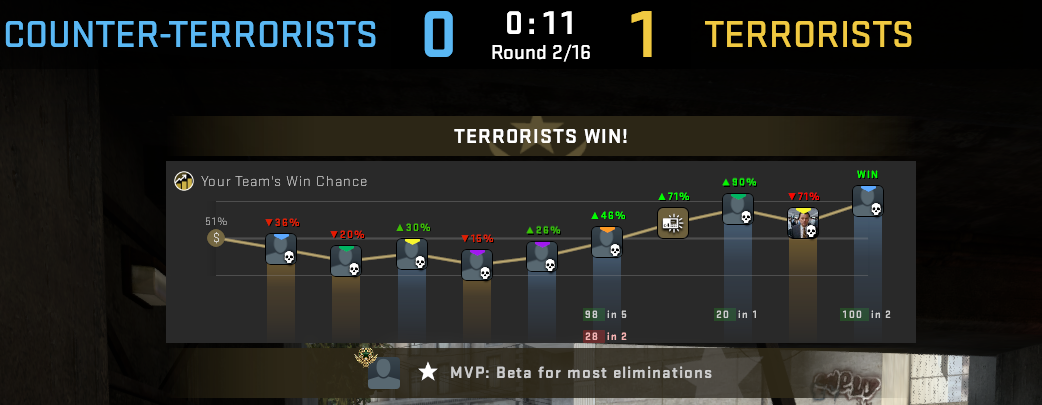
\includegraphics[width=.9\textwidth]{figures/jednanula}
 	\centering
 	\caption{CSGO graf \label{csgograf}}

 \end{figure}

 

\subsubsection{Potrebné dáta hry Counter-Strike: Global Offensive :}

 \begin{itemize}
 	\item PlayerId - unikátne ID hráča
 	\item TeamId - unikátne ID tímu hráča
 	\item OpponentId - ID opozičného tímu
 	\item Round - počet hraných kôl
 	\item MapID - ID mapy
 	\item Kills - počet zabití
 	\item Assists - počet asistencií
 	\item Deaths - počet smrtí
 	\item Headshots - počet zabití streľbou do hlavy
 	\item EntryKills - počet prvých zabití v kole počas hry
 	\item Winner - víťaz
\end{itemize}
 

 

 \subsubsection{Vyhodnotenie Counter-Strike: Global Offensive}
 Pri vyhodnocovaní použiteľnosti hry sme sa pozerali na 3 oblasti. \\ \\ Potenciál/veľkosť publika a stávkovania. Efektívnosť využitia umelej inteligencie. Dostupnosť, respektíve využiteľnosť dát z hier. \\ \\
 Z hľadiska obecenstva, dostupnosti a možnosti stávkovania je CSGO veľmi lukratívna možnosť. Databáza hráčov je rozsiahla nielen v šírom počte, ale aj v rozmanitosti pôvodu hráčov, či už Európy, Ázie alebo Ameriky. Faktom je tiež, že ju spravuje firma Valve, ktorá má na starosti veľa iných hier a zároveň spracuváva jednu z najväčších online platforiem pre virtuálnu knižnicu hier. \\
 Využiteľné dáta by sa skladali z predošlých stretnutí daných dvoch tímov, z aktuálnych informácií o jednotlivých hráčoch a ich štatistiky na vybraných mapách. Výhernosť tímu A proti tímu B a premostenie týchto informácií voči tímu C.\\
 Existuje ešte množstvo iných druhov dát, ktoré by zvýšili presnosť predikcie, ale sú to dáta, ktoré je možné zistiť už iba počas prebiehajúceho zápasu a vzhľadom na to, že stávky sa uzatvárajú pred začatím zápasu, sú tieto dáta nedostupné.
  Existuje ešte množstvo iných druhov dát, ktoré by zvýšili presnosť predikcie, ale sú to dáta, ktoré je možné zistiť už iba počas prebiehajúceho zápasu a vzhľadom na to, že stávky sa uzatvárajú pred začatím zápasu, sú tieto dáta nedostupné.
 \\ \\
 Potrebné dáta môžeme získať na stránke : \footnote {
 https://sportsdata.io/developers/data-dictionary/csgo
}


\subsection{Dota 2}
Dota je jednou z dvoch najznámejších MOBA hier na svete, s priemerným počtom hráčov viac ako 400 tisíc. \cite{dotaplayers} Podobne ako Counter-Strike má predmety a verejný trh. Na druhej strane výherný rozpočet sa s ním nedá porovnať, pretože v roku 2021 prekonal 40 miliónov, čo je jeden z najväčších zo všetkých hier na svete. \cite{dotaprizepool}
\\ \\
Dota má nástroj na vyhľadávanie hier. Na obrázku \ref{dota1} si vieme vybrať šampiónov pre oba tímy a následne nám vybehnú zápasy, ktoré prebehli s týmito podmienkami.
Po rozkliknutí zápasu si v zázname vieme pozrieť výhercu a všetky informácie sprevádzajúce daný zápas, ako môžeme vidieť na obrázku \ref{dota2}
 \begin{figure}[h!]
	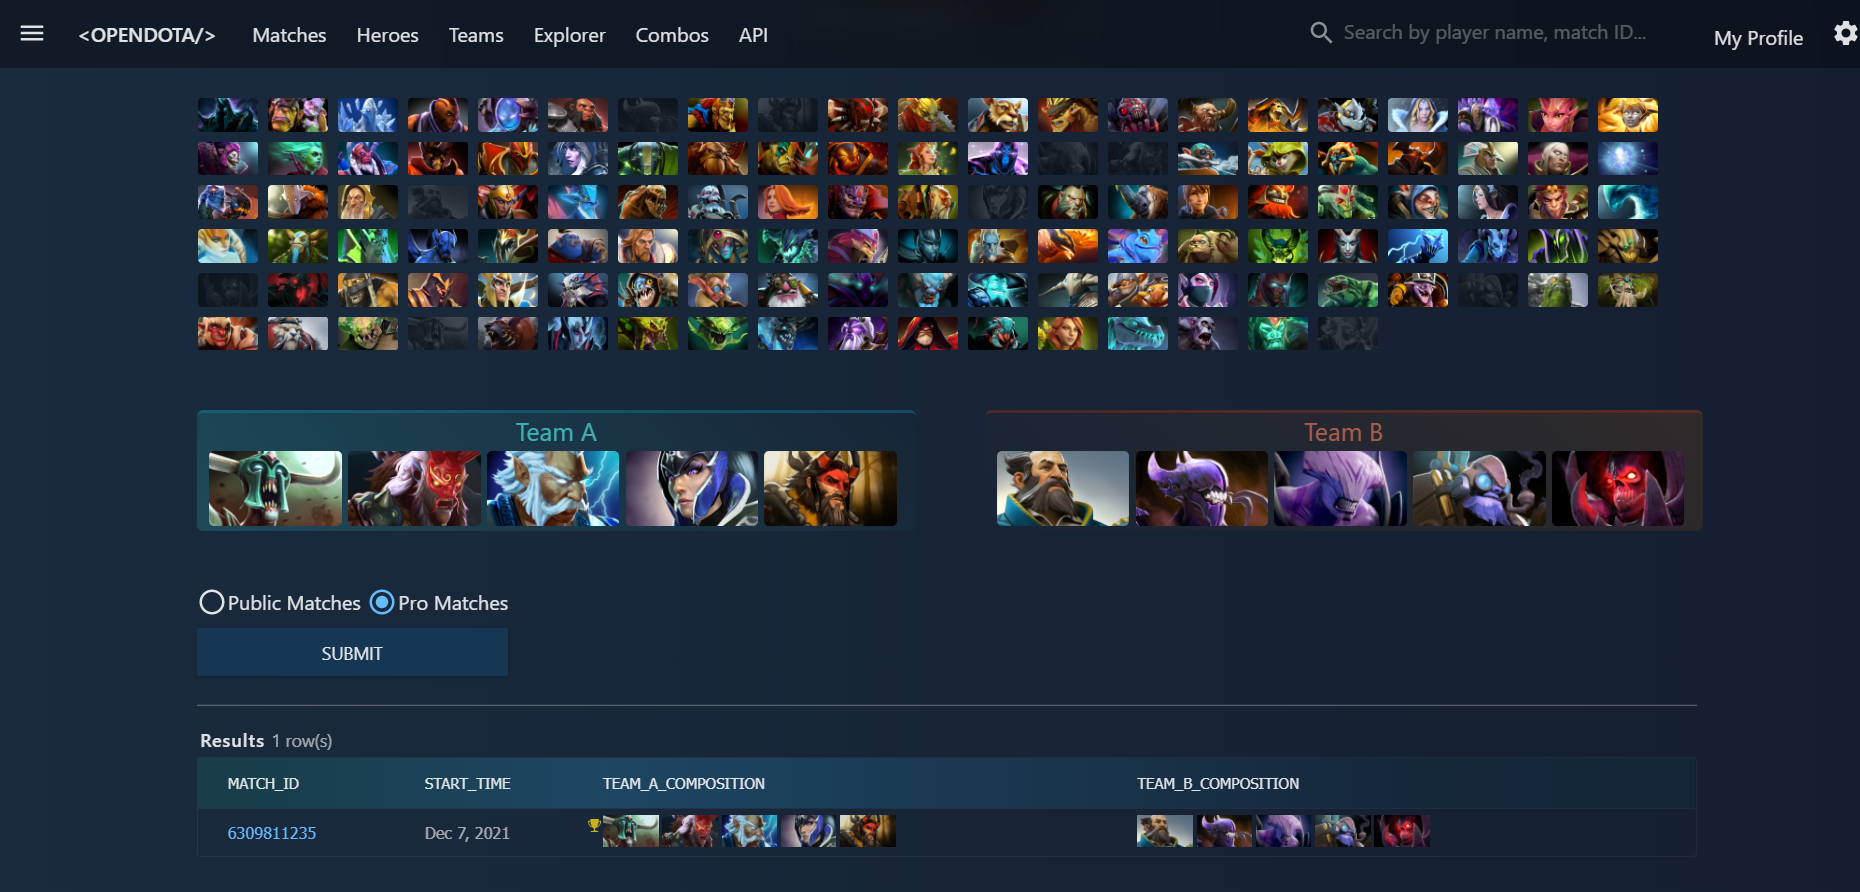
\includegraphics[width=.9\textwidth]{figures/dota1}
	\centering
	\caption{ dota1 \label{dota1}}
	
\end{figure}


 \begin{figure}[h!]
	
	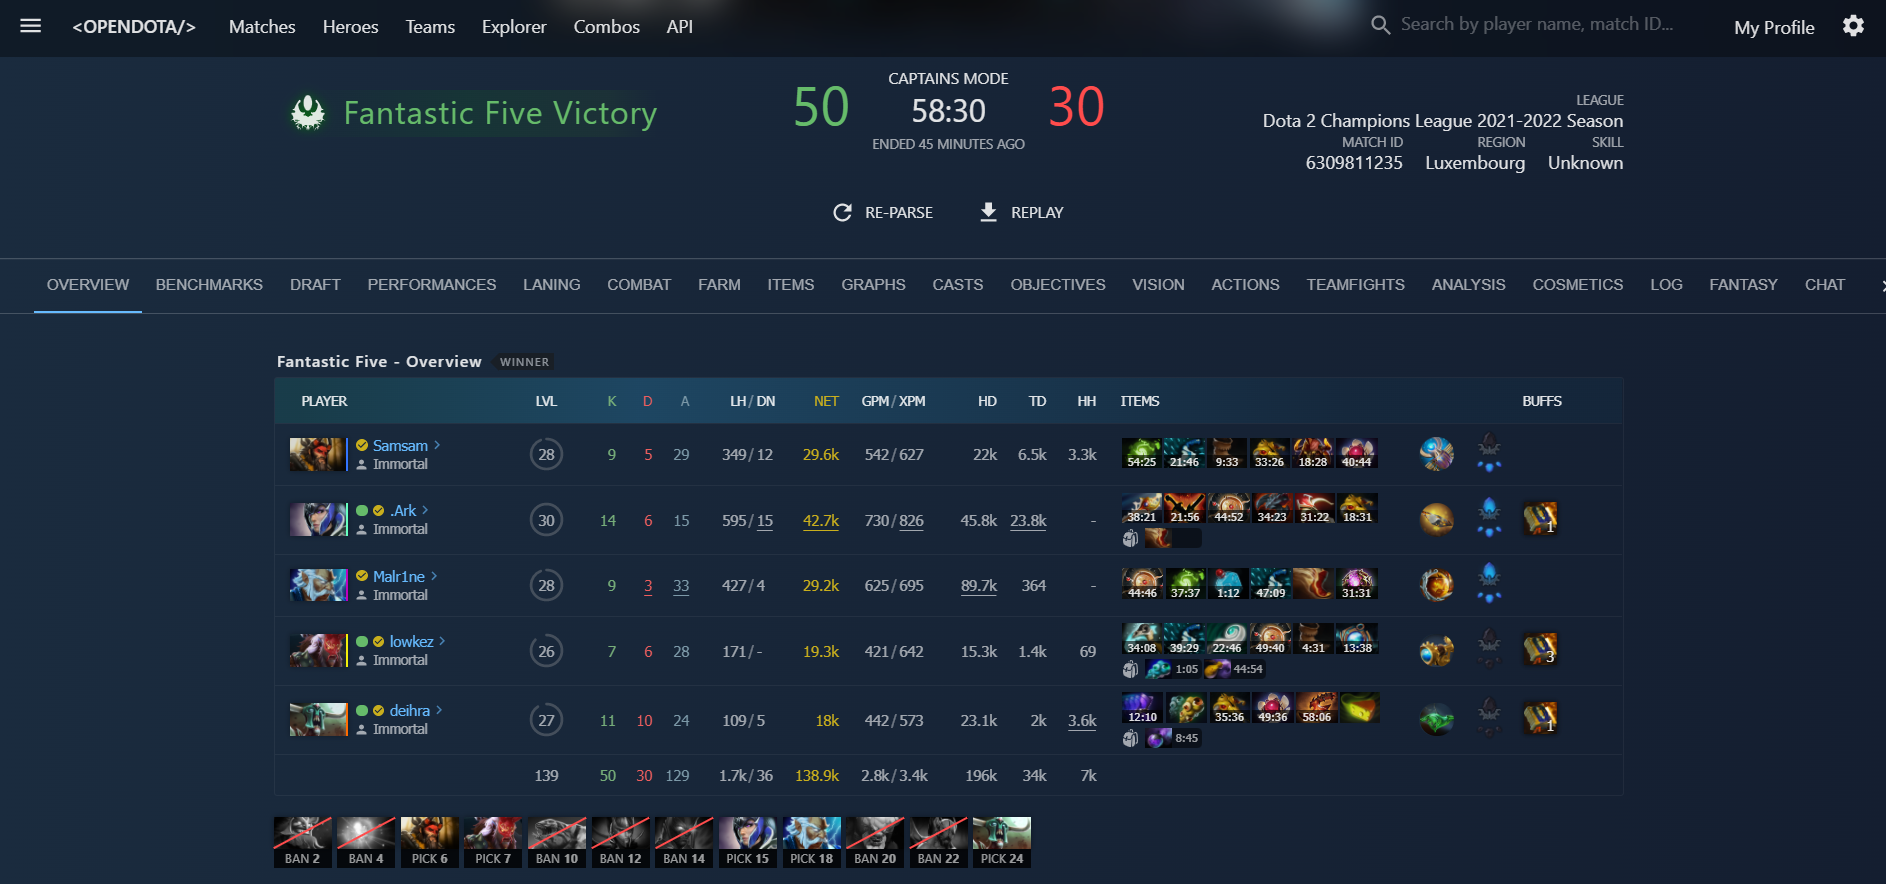
\includegraphics[width=.9\textwidth]{figures/dota2}
	\centering
	\caption{ dota2 \label{dota2}}
	
\end{figure}

\subsubsection{Dáta hry Dota 2}

 \begin{itemize}
\item match\_id - unikátne ID zápasu 
\item duration - dĺžka zápasu 
\item start\_time - začiatok zápasu 
\item radiant\_team\_id - ID radiant tímu 
\item radiant\_name - meno radiant tímu 
\item dire\_team\_id - ID dire tímu 
\item dire\_name - meno dire tímu 
\item leagueid - ID ligy
\item league\_name - meno ligy
\item series\_id - ID série
\item series\_type - typ série
\item radiant\_score - skóre radiant
\item dire\_score - skóre direy
\item radiant\_win - výherca
\item name - meno hráča
\item radiant\_picks - radiant vybraní šampióni
\item radiant\_bans - radiant zabanovaní šampióni
\item dire\_picks - dire vybraní šampióni
\item dire\_bans - dire zabanovaní šampióni
\end{itemize}

\subsubsection{Vyhodnotenie hry Dota 2}
Znovu sa pozrieme na 3 oblasti. \\ \\ 
Publikum Doti a dosah je v porovnaní s CSGO nižší, na druhej strane jeho hráči sú odhodlaní brániť ju za každú cenu, čo môže mať negatívny, ale aj pozitívny efekt. Vzhľadom na  Potenciál/veľkosť publika a stávkovania. Efektívnosť využitia umelej inteligencie a dostupnosť, respektíve využiteľnosť dát z hier.
\\ \\
Dáta pri Dote môžeme rozdeliť na dve kategórie : 
\\ \\
1. Dáta na predpoveď pred vybratím šampiónov : \\
Tieto dáta sú obmedzené z dôvodu, že nevieme akých šampiónov budú dané dva tímy hrať. Takže sa spoliehame na predošlé výsledky daných dvoch tímov a ich stretnutí navzájom alebo s podobnými tímami. Takisto, ak sú noví hráči v tíme, vieme sa pozrieť aj na dáta individuálnych hráčov a na ich stretnutia z predošlých tímov. \\
Ďalšia podmienka, ktorou by sa dala predikcia vylepšiť, vychádza z porovnaní dát hráčov v danom tíme a šampiónov, ktorí sú práve v turnaji alebo v Patchi najviac hraní. Napríklad práve v rotácii najhranejších Carry šampiónov na profesionálnej scéne je daných 10 a týchto 10 porovnáme s hráčom v Carry pozícii, koľko má za nich nahraných profesionálnych hier alebo na ich SoloQ \footnote {
	SoloQ - zápasy odohrané na serveroch so všetkými hráčmi, aj neprofesionálnymi
} účte a ich výhernosť/gold per minute/KDA(Kills, deaths, assists ratio) s týmito šampiónmi.  
\\ \\
2. Dáta na predpoveď po vybratí šampiónov : \\
Týchto dát je kvantum, lebo vieme použiť dáta o šampiónoch nie len z profesionálnych hier, ale aj z hier normálnych hráčov z vyšších líg v pomere hodnotenia, inak povedaného hodnotiaceho rebríčka. Vedeli by sme použiť dáta aj z nižšie postavených hráčov Doty, ale to by s vysokou pravdepodobnosťou zhoršilo výsledok predikcie vzhľadom na fakt, že hra top 80 percent hráčov a hra top 0.003 percent hráčov sa nedá porovnať. Veľmi dôležité informácie by teda boli o výkonnosti šampiónov ako gold per minute/average KDA alebo winrate. Zároveň by bolo veľmi zaujímavé skombinovať kompatibilnosť šampiónov spolu, spojením dvoch alebo viacerých šampiónov a ich spoločný priemerný winrate.


\subsection{League of Legends}
League of Legends(Liga Legiend) je najrozšírenejšia MOBA hra na svete s viac ako 3 miliónmi každodenných používateľov a viac ako 100 miliónmi mesačných používateľov primárne z Číny, ako môžeme vidieť na grafe : \ref{leaguegraph} 

 \begin{figure}[h!]
	
	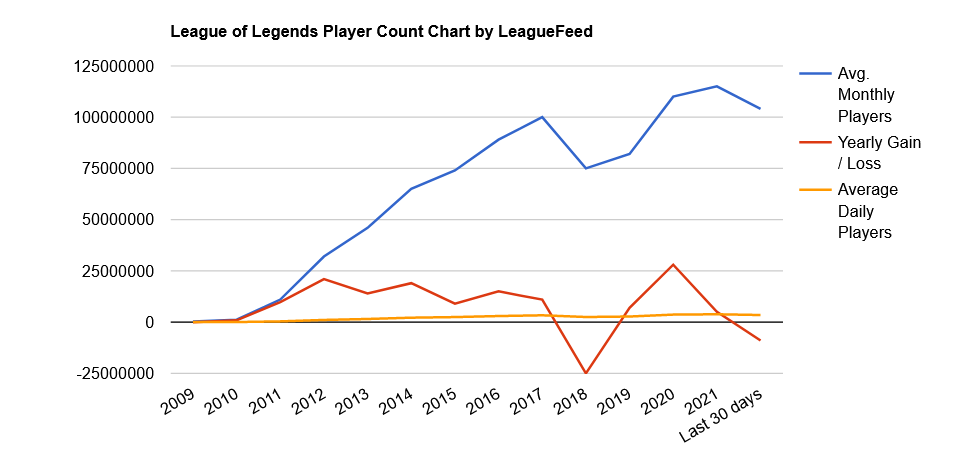
\includegraphics[width=.9\textwidth]{figures/leaguegraph}
	\centering
	\caption{ LoL graf  \label{leaguegraph}}
	
\end{figure}

Viac informácií nájdeme v článku :\cite{leaguefeed} 

Hra je z pohľadu tretej osoby a delí sa na dva tímy po piatich hráčoch. Víťazný tím je ten, ktorý zničí nepriateľskú základňu. Hráči zabíjaním nepriateľských minionov dostávajú peniaze, ktoré môžu využiť na zlepšenie ich výzbroje, čo im dá väčšiu šancu na zabitie nepriateľa a následne nepriateľskej základne.
\\ 
Riot games má podobne ako Dota verejne dostupné informácie pre developerov na stránke : 
\\ 
https://developer.riotgames.com/  
\\
a informácie o profesionálnych zápasoch na :
\\
https://lol.fandom.com/wiki/League\_Championship\_Series

\subsubsection{Dáta hry League of Legends}
\begin{itemize}
\item date - dátum zápasu 
\item blueteam - meno modrého tímu 
\item redteam - meno červeného tímu 
\item winner - víťaz 
\item bluebans - bany modrého tímu 
\item redbans - bany červeného tímu 
\item bluepicks - vybraní šampióni modrého tímu 
\item redpicks - vybraní šampióni červeného tímu 
\item blueroster - hráči modrého tímu 
\item redroster - hráči červeného tímu 
\end{itemize}
\subsubsection{Vyhodnotenie hry League of Legends}

Publikum z našich 3 hier ma LOL definitívne najväčšie, a to hlavne z dôvodu masívnej popularity v Číne, kde League of Legends má väčšiu popularitu a prestíž ako hocijaké iné, či už športy, hudba, tanec alebo spev. \cite{chinalol} 
\\
Aktuálne rozšírenie stávkovania na víťazný tím nie je vzhľadom na veľkosť publika až také rozšírené ako pri Dote a Lolku. To môže ovplyvňovať aj fakt, že gambling je v Číne vysoko ilegálny, až na výnimky ako mesto Macau.\cite{chinagambling}
\\
Využitie  umelej inteligencie v Lolku je veľké vzhľadom na verejne dostupné dáta a hlavne vysokú využiteľnosť.
\\
Dáta sú primárne veľmi podobné Dote, kde ich rozdeľujeme na dve časti, pred a po vybratí šampiónov.
\\
Veľmi lukratívne dáta, ktoré sú nanešťastie zatajené pred verejnosťou, sú dáta z hier, nazvané scrims. Pred oficiálnym začatím, napríklad svetového turnaja, sú všetky tímy zvolané a prítomné v usporiadajúcej krajine. Približne 3 týždne tieto tímy hrajú medzi sebou tréningové alebo kondičné zápasy, ktoré nie sú hodnotené, ale obsahujú veľa dôležitých informácií a taktík, ktoré tímy odskúšavajú. S prístupom k týmto dátam by sa dalo odskúšať veľa nových predikcií, ale k týmto dátam majú prístup len dané tímy a dáta sú vysoko chránené. Jedinou možnosťou, ako sa k nim dostať, by bol povolený prístup od tímov alebo odkúpenie za veľa peňazí.
\\


\section{Analýza dostupných spracovaní dát}
Časť analýzy dostupných spracovaní dát sa bude venovať jednotlivým druhom umelej inteligencie.

\subsection{Supervised learning}
Podkategória umelej inteligencie, ktorá používa daný dataset na natrénovanie modelu.

\subsection{Reinforcement learning}
Časť umelej inteligencie, pri ktorej sa sledujú kroky inteligentných agentov na maximalizáciu efektívnosti dosiahnutia cieľa.

% !TEX root = ../thesis.tex

\chapter{Syntetická časť}
\label{methodology}

Syntetická časť opisuje metódy použité na syntézu riešenia a opisuje syntézu samotného riešenia (zvyčajne je to návrh/implementácia softvérového resp. hardvérového riešenia), pričom sa opiera o~závery analytickej časti práce. Začína od toho, ako sa bude riešenie používať: najdôležitejšie scenáre používania a používateľské rozhranie, ktoré bude tieto scenáre efektívne podporovať. Až potom je na rade vnútorná architektúra alebo použité technológie. Syntetická časť tvorí zvyčajne ½ jadra práce.

Syntetickú časť práce vhodne rozdeľte do kapitol a pomenujte ich podľa toho, čomu sú venované.

% !TEX root = ../thesis.tex

\chapter{Vyhodnotenie}
\label{evaluation}
Vo vyhodnocovacej časti by sme sa chceli venovať bližšiemu pohľadu na výsledky testovania.

\section{Testovanie}
Pri testovaní sme použili 58 profesionálnych zápasov, to znamená známku sme pridávali 116 rôznym kombináciám. Ani jedna tímová zostava nebola rovnaká. Najnižšie získané skóre bolo 44,9249, na druhej strane najvyššie získané skóre bolo 55,5978. Tím s najnižším pridaným skóre prehral a tím s najvyšším skóre vyhral, čo je na začiatok celkom povzbudzujúce. 
\\Priemerné skóre tímov, ktoré vyhrali, bolo 51,6450, toto skóre je priamo na hranici známky B. 
\\Priemerné skóre tímov, ktoré prehrali, bolo 50,6645, toto skóre je priamo na hranici známky C.
\subsubsection{Rozdiely medzi tímami}
Na obrázku \ref{rozdiel} je znázornené, aký rozdiel bol medzi víťazným tímom a tímom, ktorý prehral. \\Všetky prípady nad rovinou 0 označujú prípady, pri ktorých náš model určil lepšiu známku tímu, ktorý vyhral, pričom najväčší rozdiel bol 9,3176.
\\ Na druhej strane všetky prípady pod nulou označujú inštancie, kedy zvíťazil tím, ktorý náš model určil ako znevýhodnený, tu bol najväčší rozdiel -3,7837.
\\ Priemerný rozdiel bol v súlade s naším modelom a to 0,9804, čo označuje skoro celotriedový rozdiel.
\begin{figure}[h!]
	
	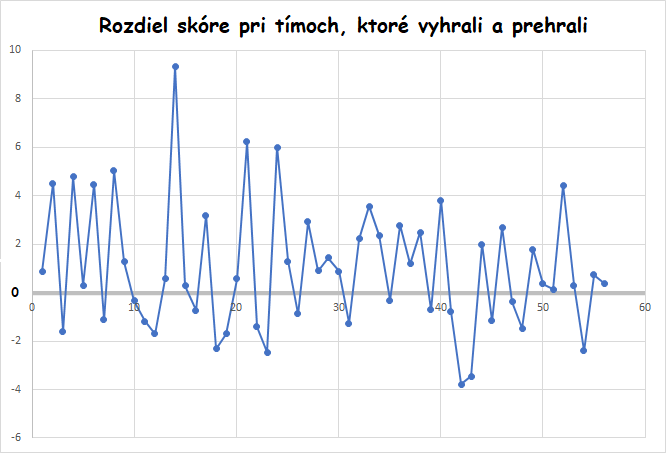
\includegraphics[width=.9\textwidth]{figures/rozdiel}
	\centering
	\caption{ Rozdiel pridaných skóre pri tímoch \label{rozdiel}}
	
\end{figure}

\subsubsection{Známkovanie testovaných tímov}
Pri určovaní známok sme použili tabuľku, o ktorej sme rozprávali v minulej časti. 
\\ \\
Ako môžete vidieť na obrázku \ref{win}, výsledky tímov, ktoré vyhrali, mali všetky prípady, kde tím dostal hodnotenie S+, čo boli 4 tímy. Na druhej strane 1 tím, ktorý vyhral, dostal známku F, konkrétne im bolo pridané skóre 47,9589, čo je na hranici medzi F a E, takisto tím, ktorý porazili, bol ohodnotený známkou D, čo nie je až taký veľký rozdiel a je to predvídateľné.
\\
Väčšina víťazných tímov skončila so známkou B a C, pričom 8 tímov dostalo známku S.
\begin{figure}[h!]
	
	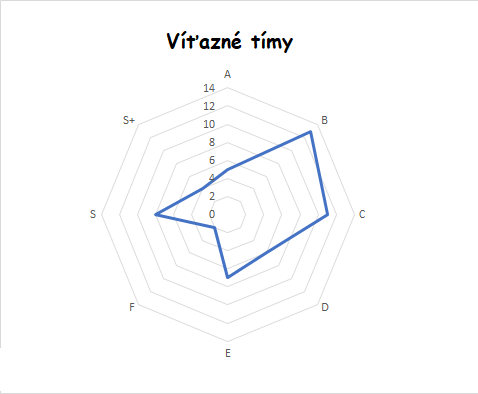
\includegraphics[width=.9\textwidth]{figures/win}
	\centering
	\caption{ Známkovanie víťazných tímov \label{win}}
	
\end{figure}
\\ \\
Na obrázku \ref{lose} vidíme oznámkovanie tímov, ktoré prehrali ich súboj. Najvyššie oznámkovanie bolo S, kde 3 tímy označené druhou najlepšou známkou S prehrali, konkrétne prehrali proti tímom označeným C, B a D. Zhodou okolností súboj tímu S a D bol prípad najväčšieho rozdielu, kde náš model určil nesprávneho víťaza. Rovnako 6 tímov označených známkou A prehralo proti tímom S+, S, S, B, C, D.
\\ 
Najväčšia porcia tímov, ktoré prehrali dostala známku D, C a E, pričom 10 tímov dostalo známku B.

\begin{figure}[h!]
	
	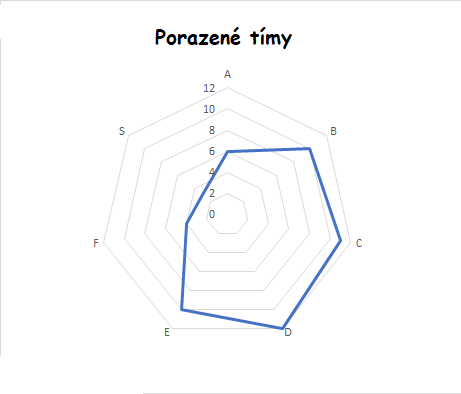
\includegraphics[width=.9\textwidth]{figures/lose}
	\centering
	\caption{ Známkovanie porazených tímov \label{lose}}
	
\end{figure}

\section{Zhodnotenie výsledky testovania}
Výsledky sú lepšie, než sme predpokladali. Je značný rozdiel v tímových kompozíciach, ktorý náš program vie rozoznať.
\\
V testovacej časti sme odhalili, že v 58 prípadoch bolo 31, kde náš program dal víťaznému tímu lepšiu známku, čo reprezentuje 54 percent zo všetkých prípadov.
V 14 prípadoch dostal lepšiu známku tím, ktorý prehral, čo označuje približne 24 percent z celkových prípadov.
V ostatných 13 prípadoch dostali tímy rovnakú známku, čo je približne 22 percent z prípadov.
\\ 
Čo znamená, že ak budeme tipovať na tímy, ktoré majú rozdielne známkovanie, tak máme približne 68,89 percentnú šancu, že náš program dá lepšiu známku tímu, ktorý zápas vyhrá.

% !TEX root = ../thesis.tex
\chaptermark{summary}
\phantomsection
\chapter{Záver}
\label{summary}
Na začiatku našej práce nám nebolo úplne jasné, ako dosiahneme náš cieľ, no vedeli sme, že chceme zlepšiť šancu na úspešné tipovanie víťazného tímu. Naše obzory a ciele sa ale počas pracovania na tejto práci zmenili a uvedomili sme si nielen potenciál, ale aj viacero obmedzení.
\\
Primárne vnímame 2 hlavné využitia. 
\begin{itemize}
	\item Prvé využitie spočíva pri stávkovaní. Je malé okienko času medzi vybratím šampiónov a začiatkom hry. Ak by sme stihli zadať a oznámkovať kompozície v tomto čase a výsledky by určili 2 rôzne známky, tak máme možnosť staviť na tím, ktorý má lepšiu známku. Ak by sme používali túto techniku počas viacerých zápasov, malo by to byť výnosné, no negarantujeme výsledky, stále je veľa ovplyvňujúcich faktorov, ktoré sa často krát nedajú zarátať.
	\item Druhé využitie by bolo v práci analytika. Tak isto, ako veľké firmy majú analytikov, ktorí spracovávajú veľké množstvo dát na zlepšenie chodu ich firmy, majú aj profesionálne tímy členov, ktorí sa venujú analýze. Títo analytici by mohli využiť náš program na zlepšenie ich pohľadu na hru a zároveň určenie typov kompozícií, ktoré sú efektívne. Áno, analytici majú presnejší pohľad na hru, ale ich myseľ nie je dostatočná na spracovanie stá-tisíc hier, čo ale náš program dokáže.
\end{itemize}




% good linebraking of bibtex url
\setcounter{biburllcpenalty}{7000}
\setcounter{biburlucpenalty}{8000}

%% The bibliography
\printbibliography[heading=bibintoc]

\label{theend} % the last page of the thesis

% List of acronyms
\printglossary[type=\acronymtype,title={\acrlistname}]

% Glossaries
\printglossary

%% Appendix
% !TEX root = ../thesis.tex

\chapter*{Zoznam príloh}
\addcontentsline{toc}{chapter}{Zoznam príloh}

\begin{description}
	\item[Príloha A] Karel Language Reference
    \item[Príloha B] CD médium -- záverečná práca v~elektronickej podobe,
    \item[Príloha C] Používateľská príručka
    \item[Príloha D] Systémová príručka
\end{description}

\appendix
\renewcommand\chaptername{Príloha}
% !TEX root = ../thesis.tex

\chapter{Systémová príručka}
Táto časť slúži na opis priečinkov a rozdelenia kódu.
\section*{Rozdelenie kódu}
Funkčný kód je rozdelený na dve časti. Prvá časť sa venuje základnej úprave dát do čitateľnej formy, konkrétne vo funkcii main napísanej v kóde java. Druhá časť, ktorá klasifikuje všetky dáta, spracováva výsledky a vypočítava skóre, je napísaná v Pythone, konkrétne v main funkcii predict.py. 
\section*{Opis kódu}
Prvá časť v kóde main.java má dve funkcie. Je to funkcia GetCharFromString, ktorá vracia aktuálny charakter v stringu a funkcia main, v ktorej otvoríme ako BufferedReader textový súbor 'menochampiona'+1.txt a zároveň vytvoríme nový textový súbor 'menochampiona'+.txt. Následne prechádzame celý textový súbor a upravujeme ho do čitateľnej podoby.
\\ Druhá čast v kóde predict.py má dve hlavné priority. Prvá je zápis všetkých získaných textových súborov z programu javy do jedného dataframu a zároveň ich klasifikácia. A druhá pracuje s daným dataframom a počíta skóre.
\section*{Opis priečinkov}
V priečinku transformdata sa nachádza 332 súborov, z čoho je viac než 320 textových súborov s dátami o každom jednom šampiónovi. Zároveň je tam aj hlavná časť kódu a to súbor predict.py, ktorý má v sebe spracovanie a úpravu všetkých dát. Hlavný súbor s dátami sa volá winratedata.txt ktorý v sebe drží hodnoty všetkých klasifikovaných dát pre každého šampióna. Takisto v hlavnom priečinku môžete nájsť vysledky.xlsx, čo je excelovská tabuľka všetkých otestovaných zápasov. V priečinku src nájdeme kód main.java, pomocou ktorého sme dáta dostali do čitateľnej podoby pre náš python kód. 

\chapter{Používateľská príručka}
V tejto časti si ukážeme ako spustiť a obsluhovať aktuálny kód.

\section*{Potrebné súbory}
Na úspešné odskúšanie kódu na predikciu potrebujete mať textové súbory winratedata.txt, winlose.txt, teams.txt a zároveň samotný súbor s kódom predict.py, ktorý sa nachádza v hlavnom priečinku spolu s textovými súbormi.

\section*{Príprava prostredia a knižníc} 
Odporúčané prostredie je Spyder, ideálne verzia 5.0.5 a novšie. Prostredie Spyder je možné stiahnuť na ich domácej stránke zadarmo. Potrebná knižnica na stiahnutie je pandas, čo môžete vykonať príkazom - pip install pandas, napísaným v konzole.

\section*{Popis používania}
Kód predict.py je potrebné otvoriť v predpripravenom prostredí. Následne na vrchu kódu je 5 premenných top, jg, mid, bot a sup. Pri predikcii kompozície, ktorú chcete odskúšať do týchto premenných, vložte mená šampiónov bez medzier v ich mene s malými písmenami. Ak ste tak vykonali, spustite kód zelenou šípkou a v konzole by mali byť vypísané premenné totalgames, totalscore a známka, čo označuje aktuálnu kompozíciu, ktorú ste zapísali. 


% zivotopis autora
%\curriculumvitae\protect
%Táto časť\/ je nepovinná. Autor tu môže uviesť\/ svoje biografické
%údaje, údaje o~záujmoch, účasti na~projektoch, účasti na~súťažiach,
%získané ocenenia, zahraničné pobyty na~praxi, domácu prax, publikácie
%a~pod.

\end{document}
